\chapter{Estática de la partícula libre}	


\begin{miparrafo}
La estática es la parte de la mecánica que estudia el punto material sobre el que actúan fuerzas y momentos totales  cuyas resultantes son nulas, de forma que permanece en reposo o en movimiento rectilíneo y uniforme ($\vec v=\overrightarrow{cte}$), en equilibrio.	
\end{miparrafo}


\section{Estática del punto material. Ligaduras}

Si un \textbf{punto material, masa puntual o partícula} no tiene su movimiento impedido por ninguna restricción, decimos que es un \textbf{punto libre}. Para definir su posición en un espacio tridimensional se requiere el conocimiento de tres coordenadas, diremos que tiene tres grados de libertad, pues tiene la posibilidad de desplazarse en las tres direcciones de los ejes $X$, $Y$ y $Z$. 

Si el punto material tiene alguna limitación en su movilidad, se dice que es un \emph{punto ligado o vinculado}, y a la causa de esa limitación, se la denomina ligadura, vínculo, o \emph{enlace}.

Un punto obligado a permanecer en una línea está ligado a la misma. Su posición puede ser definida ahora por un único parámetro. Ahora el punto sólo tiene un grado de libertad, esto es, únicamente tiene la posibilidad de desplazarse en la dirección tangencial de la línea. 

Otro ejemplo: un punto obligado a permanecer en una superficie. Su posición se puede definir con dos parámetros, y tendrá dos grados de libertad. 


\colorbox{LightYellow}{\textbf{Ligadura}} de un punto material (o de un cuerpo) es cada una de las \colorbox{LightYellow}{condiciones} que se le imponen que \colorbox{LightYellow}{limitan su de movimiento}.

\vspace{4mm} %**************************
Las ligaduras pueden ser:

\vspace{-2mm} %**************************
\begin{itemize}

\item \emph{Ligaduras bilaterales o completas}:	 se pueden expresar por una \emph{igualdad matemática}.

Ejemplo: $x^2+y^2+z^2=r^2 \to $ la partícula se puede mover por una suferficie esférica de radio $r$.

\item \emph{Ligaduras unilaterales o incompleta}s: se pueden expresar por medio de \emph{desigualdades matemáticas}.

Ejemplo: $x^2+y^2+z^2 \le r^2 \to $ la partícula se puede mover por el interior de una esfera de radio $r$.

\end{itemize}

\vspace{-4mm} %**************************
\begin{figure}[H]
	\centering
	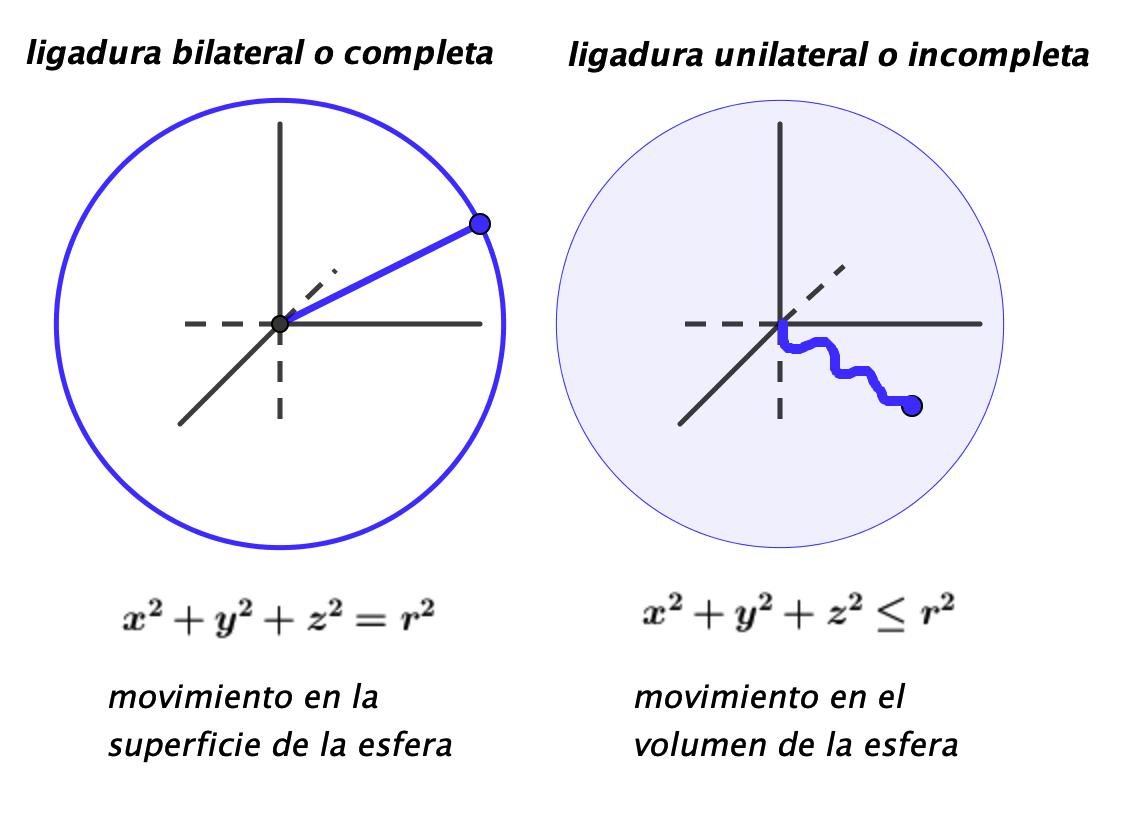
\includegraphics[width=.7\textwidth]{imagenes/imagenes05/T05IM01.png}
	\caption*{Tipos de ligaturas.}
\end{figure}

\section{Principio de las fuerzas de ligadura}

Consideremos un cierto punto material, sometido a una cierta ligadura o enlace y sobre el que actúan una serie de fuerzas, cuya resultante es $\overrightarrow{F}$ . 

Si dicho punto está  ligado y por lo tanto tiene su movilidad impedida de algún  modo, no asumirá por efecto de la fuerza  $\overrightarrow{F}$ el mismo movimiento que si dicho punto estuviese libre, por lo que las ligaduras que actúan sobre los puntos materiales, pueden ser equiparables a fuerzas.
 
 De este planteamiento se deriva el principio de las fuerzas de ligadura: 

\emph{En un punto material ligado, la acción de las ligaduras,  se puede sustituir por la de una fuerza que llamaremos fuerza reactiva o de ligadura}. 

\begin{itemize}
\item Estas fuerzas reactivas o de ligadura tienen unas características propias que las diferencian de las fuerzas aplicadas: 
\item Las fuerzas de ligadura dependen de las fuerzas aplicadas. 
\item Si las fuerzas aplicadas se anulan, las fuerzas de ligadura también se anulan, incapaces por sí mismas de producir movimiento. 
\end{itemize}

\vspace{-5mm} %*******************************
$$\text{fuerza de ligadura } + \text{ fuerza aplicada }\to \text{ trayectoria de la partícula}$$



\section[Ecuaciones de equilibrio de la partícula libre]{Ecuaciones de equilibrio de la partícula libre\sectionmark{Ecuaciones de equilibrio de la partícula libre}}
\sectionmark{Equilibrio de la partícula libre}

Desde el punto de vista de la estática, un cuerpo libre es aquel que puede moverse en cualquier dirección y sentido, el que no está sujeto a ligaduras. (Dinámicamente, dos cuerpos son libres cuando la distancia que les separa es infinita, cuando no interaccionan.)

Un cuerpo se encuentra en equilibrio si las fuerzas que actúan sobre él lo mantienen inmóvil o en movimiento rectilíneo y uniforme. Las condiciones de equilibrio se deben dar respecto de un determinado observador.

Condiciones de equilibrio:
\begin{enumerate}
\item $\vec v_{observador}=\vec 0$
\item $\displaystyle \overrightarrow{F}_{total}=\vec 0=\sum_{i=1}^N \vec F_i$	

Lo que implica: $\displaystyle \sum_{i=1}^N \vec F_{x_i}=0;\quad \sum_{i=1}^N \vec F_{y_i}=0;\quad \sum_{i=1}^N \vec F_{z_i}=0$
\end{enumerate}


Como caso particular vamos a estudiar las condiciones de equilibrio de un punto material (partícula) en una región del espacio en que hay un \textbf{campo conservativo.}


Es trivial que $\vec v=\vec 0$. Vamos con la fuerza: $\overrightarrow{F}=0=-\overrightarrow{\grad}{\mathcal E_p} \to $

$$\displaystyle \pdv{\mathcal E_p}{x}=0;\quad \pdv{\mathcal E_p}{x}=0;\quad \pdv{\mathcal E_p}{z}=0;\qquad \mathcal E_p=\mathcal E_p(x,y,z)$$

\begin{miparrafodestacado}
	En un campo conservativo, una partícula está en equilibrio cuando ocupa un máximo o un mínimo de energía potencial. (Si en un punto hay un máximo o mínimo, la derivada en él es cero.)
\end{miparrafodestacado}






\begin{figure}[H]
	\centering
	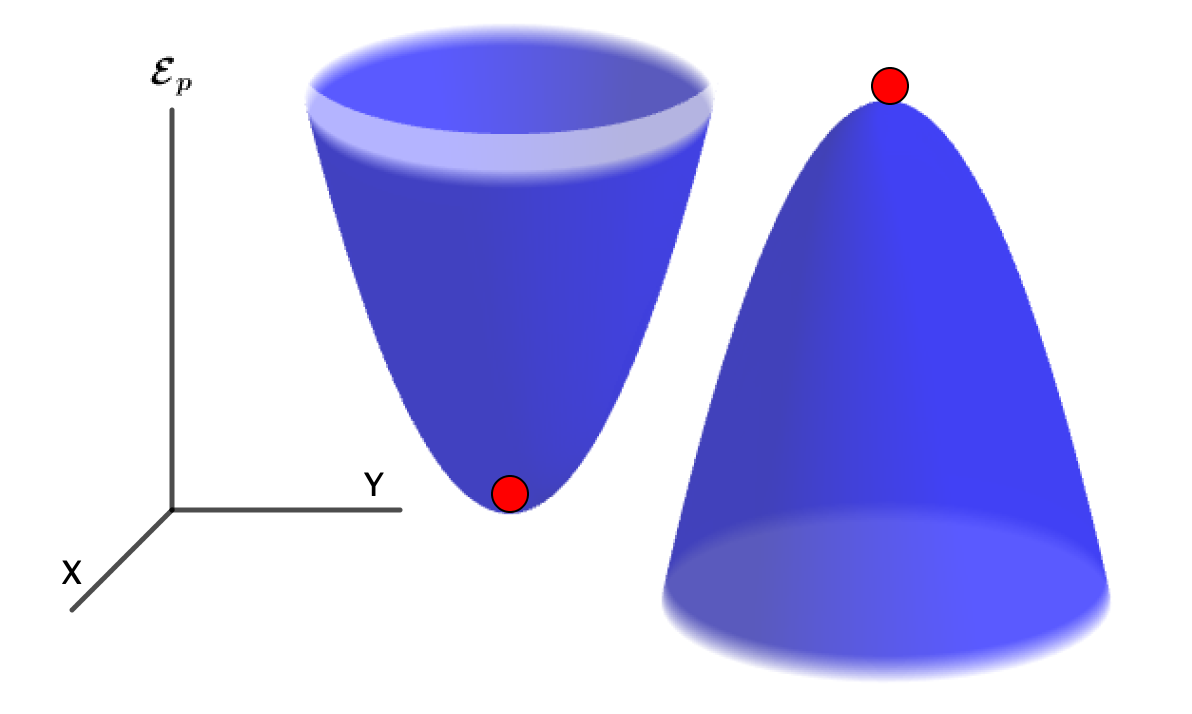
\includegraphics[width=.75\textwidth]{imagenes/imagenes05/T05IM02.png}
\end{figure}

\section{Teorema de Lejeune Dirichlet}
\label{Lejeune-Dirichlet}

\emph{Siempre que el campo que actúe sobre una partícula derive de un potencial (esto es, que sea un\colorbox{LightYellow}{ campo conservativo}) la condición necesaria y suficiente para que el la partícula esté en \colorbox{LightYellow}{equilibrio} es que en dicho punto exista un \colorbox{LightYellow}{máximo o mínimo para la energía potencial}; siendo el equilibrio \colorbox{LightYellow}{inestable} en el primer caso y \colorbox{LightYellow}{estable} en el segundo.}

Se dice que un cuerpo está en \emph{equilibrio estable} cuando al separarlo de esa posición una distancia infinitesimal, aparece aplicada sobre él una fuerza que tiende a restablecer el equilibrio, a devolver a la partícula a su posición inicial.

Una partícula ocupa una posición de \emph{equlibrio inestable} cuando al separarla una cantidad infinitesimal de esa posición aparece una fuerza que tiende a alejarla de ella infinitamente.

El \emph{equilibrio} es \emph{indiferente} cuando no depende de la posición de la partícula.

Vamos a demostrar que:
\vspace{-3mm}
\begin{quotation} % SANGRADO ************************
	$\begin{array}{lcl}
\text{energía potencial es máxima }&\to&\text{ equilibrio es INESTABLE}	
\\
\text{energía potencial es mínima }&\to&\text{ equilibrio es ESTABLE}		
\end{array}$
\end{quotation}

\begin{figure}[H]
	\centering
	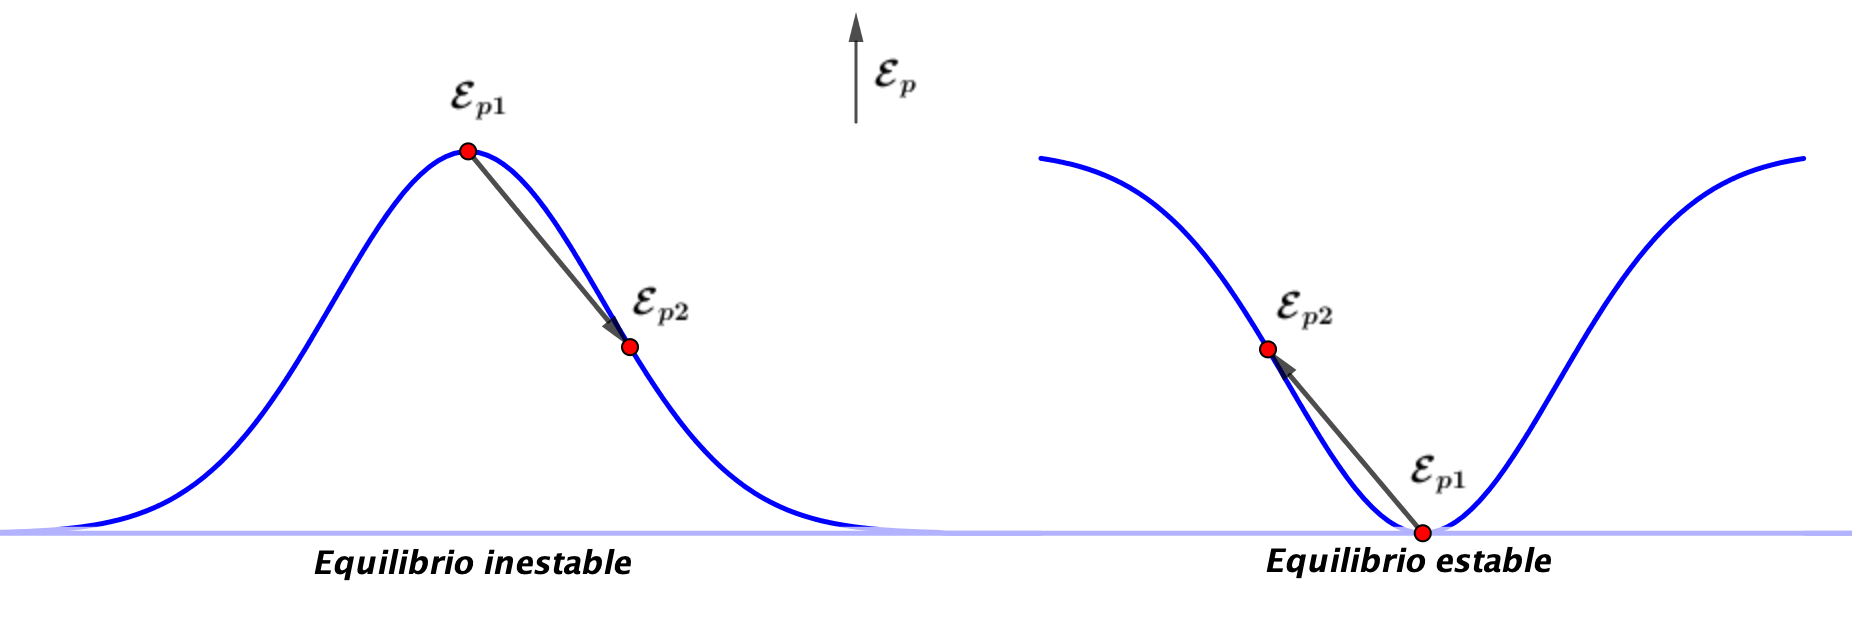
\includegraphics[width=.9\textwidth]{imagenes/imagenes05/T05IM03.png}
\end{figure}

Como vimos en la sección \ref{potenciales-decrecientes}, al ser la fuerza el \emph{menos} gradiente de la energía potencial, estará orientada hacia potenciales decrecientes (y es perpendicular a las superficies equipotenciales), por ello:

--- $\mathcal E_{p_1}>\mathcal E_{p_2}$, aparece una fuerza, orientada hacia potenciales decrecientes, que tiende a alejar a la partícula de la posición que ocupa.

--- $\mathcal E_{p_1}<\mathcal E_{p_2}$, aparece una fuerza, orientada hacia potenciales decrecientes, que tiende a aproxima a la partícula de la posición que ocupaba.

\section[Equilibrio de la partícula libre sometida a ligaduras]{Equilibrio sometido a ligaduras\sectionmark{Equilibrio sometido a ligaduras}}
\sectionmark{Equilibrio sometido a ligaduras}
Las ligaduras se pueden representar por \emph{fuerzas de ligaduras}.

\vspace{-3mm}$$F_{resultante}=F_{\text{aplicada, solicitante o externa}}+F_{ligaduras}$$

\vspace{-3mm}\emph{Para que una partícula ligada se encuentre en equilibrio, basta con que sean nulas las componentes de la fuerza que, de existir, darían lugar a movimientos compatibles con las condiciones de ligadura}.

\vspace{-3mm}$$\displaystyle \sum_{i=1}^N (\overrightarrow{F}_{aplicadas}+\overrightarrow{F}_{ligaduras})_i=0$$

\vspace{-3mm}Veamos dos casos particulares a modo de ejemplos:

\begin{ejem}
\textbf{Equilibrio de un punto ligado a una superficie fija}.	
\end{ejem}
\begin{figure}[H]
	\centering
	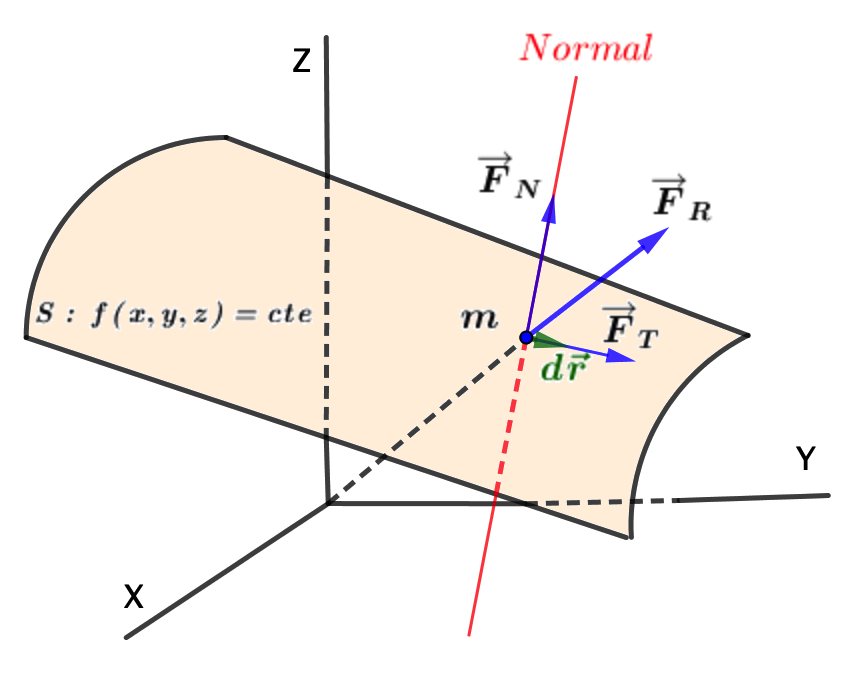
\includegraphics[width=.75\textwidth]{imagenes/imagenes05/T05IM04.png}
\end{figure}
Vamos a por las ecuaciones matemáticas que proporcionan el equilibrio:

$\overrightarrow{F}_{Resultante}= \overrightarrow{F}+\overrightarrow{N}=\vec 0 \Rightarrow \begin{cases} F_x+N_x=0\\F_y+N_y=0\\F_z+N_z=0\end{cases}$. Suponemos $\overrightarrow{F}_R=\overrightarrow{cte}$.

$f$ es la ecuación de la superficie, $f=cte \to \dd f=0 \quad \textcolor{gris}{(1*)}$:

$\displaystyle \dd f=\pdv{f}{x} \dd x+\pdv{f}{y} \dd y+\pdv{f}{z} \dd z=0\quad \textcolor{gris}{\leftarrow (1*)}$

Ecuación que vectorialmente se escribe así:

$\displaystyle \left( \vec i \ \pdv{f}{x} + \vec j \ \pdv{f}{y} +\vec k \ \pdv{f}{z} \right) \cdot \left( \vec i \ \dd x+ \vec j \ \dd y + \vec k \ \dd z \right)=0$


El primer vector le llamaremos $\overrightarrow{\lambda}=\overrightarrow{\grad}f$ y, al ser el gradiente de la función escalar que da la superficie, es perpendicular a ésta, paralelo a su vector normal: $\overrightarrow{\lambda}\ \parallel \ \overrightarrow{N}$. 

Un vector unitario en la dirección de la normal lo podemos obtener como $\vec u_N=\dfrac{\overrightarrow{\lambda}}{\lambda}$. Con esto: $\quad \overrightarrow{\lambda}=\lambda \ \vec u_N$

El segundo vector es $\dd \vec r$ y coincide con la dirección tangente del movimiento de la partícula por la superficie $S$ debido a la acción de la fuerza $F_T$.

$\vec u_N=\displaystyle \dfrac { \vec i \ \pdv{f}{x} + \vec j \ \pdv{f}{y} +\vec k \ \pdv{f}{z} }{\sqrt{ \left(\pdv{f}{x} \right)^2 + \left(\pdv{f}{y} \right)^2 + \left(\pdv{f}{z} \right)^2 }} =  \dfrac{\overrightarrow{\lambda}}{\lambda}= \vec i \ \dfrac 1 \lambda \ \pdv{f}{x} + \vec j \ \dfrac 1 \lambda \ \pdv{f}{y} +\vec k \ \dfrac 1 \lambda \ \pdv{f}{z}$


$\displaystyle \overrightarrow{N}=N\ \vec u_N=\vec i \ N_x+\vec j \ N_y+\vec k \ N_z= \dfrac N \lambda \ \pdv{f}{x} \ \vec i +  \dfrac N \lambda \ \pdv{f}{y} \ \vec j + \dfrac N \lambda \ \pdv{f}{z} \ \vec k$

$\ \displaystyle N_x=\dfrac N \lambda \pdv{f}{x} = n\ \pdv{f}{x}; \quad \displaystyle N_y=\dfrac N \lambda \pdv{f}{y} = n\ \pdv{f}{y}; \quad \displaystyle N_z=\dfrac N \lambda \pdv{f}{z} = n\ \pdv{f}{z}$, donde $\dfrac N \lambda = cte = n$

\vspace{30mm} %******************************************

\begin{multicols}{2}
$\quad$

$\quad$

Las ecuaciones de equilibrio son: 

$\quad$

(4 ecuaciones con 4ingógnitas $x,y,x$ del punto de equilibrio y $n$)

$$\displaystyle
\begin{cases}
\displaystyle \ F_x+n\ \pdv{f}{x}=0 \\ \\ \displaystyle \ F_y+n\ \pdv{f}{y}=0 \\  \\ \displaystyle \ F_z+n\ \pdv{f}{z}=0 \\ \\ \ f(x,y,z)=cte
\end{cases}$$
\end{multicols}


\begin{ejem}
\textbf{Equilibrio de un punto ligado a una curva fija}.	
\end{ejem}
\begin{multicols}{2}
	
Una curva es la intersección de dos superficies:

$Curva: \begin{cases} \ f_1(x,y,z)=\mathcal C_1 \\ \ f_2(x,y,z)=\mathcal C_2 \end{cases}$

$Equilibrio \ \leftrightarrow \ \overrightarrow{F}_{resultante}=\vec 0$

$\overrightarrow{F}+\overrightarrow{N}_1 + \overrightarrow{N}_2=\vec 0$

$\begin{cases}\ F_x+N_{1_x}+N_{2_x}=0  \\  \ F_y+N_{1_y}+N_{2_y}=0 \\ \ F_z+N_{1_z}+N_{2_z}=0 \end{cases}$
 
\begin{figure}[H]
	\centering
	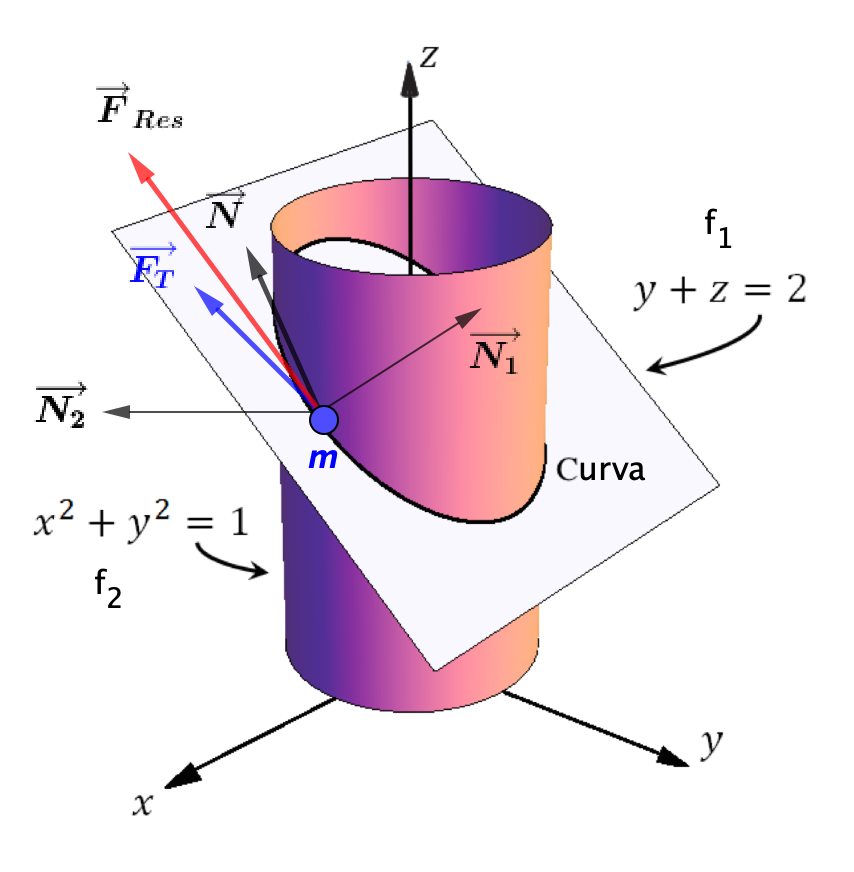
\includegraphics[width=.55\textwidth]{imagenes/imagenes05/T05IM05.png}
\end{figure}
\end{multicols}

Por un razonamiento matemático similar al anterior, las ecuaciones de equilibrio en este caso estan formadas por 5 ecuaciones con 5 incóngintas, $x,y,z,n_1,n_2$.

$$\displaystyle
\begin{cases}
\displaystyle \ F_x+n_1 \ \pdv{f_1}{x} + \ n_2\ \pdv{f_2}{x}=0 \\ \\ \displaystyle \ F_y+n_1\ \pdv{f_1}{y} + \ n_2\ \pdv{f_2}{y}=0  \\  \\ \displaystyle \ F_z+n_2\ \pdv{f_1}{z} + \ n_2\ \pdv{f_2}{z}=0  \\ \\ \ f_1(x,y,z)=\mathcal C_1 \\ \\f_2(x,y,z)=\mathcal C_2
\end{cases}$$

\section{Problemas}
\begin{prob}
Expresar matemáticamente el hecho de que una partícula se encuentre limitada a moverse en la región interna de un paralelepípedo de aristas $a$, $b$ y $c$. ?`A qué tipo de ligadura está sometida?	
\end{prob}
\begin{multicols}{2}
Colocamos el origen de nuestro sistema de referencia en uno de los vértices del paralelepípedo.

Ligadura: $\ \ \begin{cases} \ x<a \\ \ y<b \\ \ z < c \end{cases}$

La ligadura es incompleta o bilateral.
\begin{figure}[H]
	\centering
	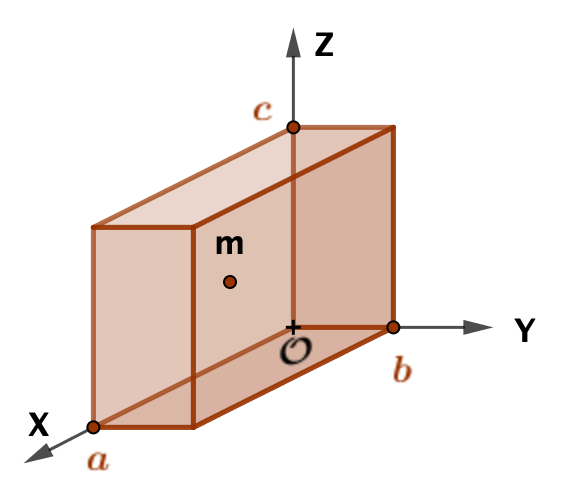
\includegraphics[width=.4\textwidth]{imagenes/imagenes05/T05IM06.png}
\end{figure}
\end{multicols}

\begin{prob}
Determínense las posiciones de equilibrios de una partícula libre atraída por $n$ centros fijos $\mathcal O_1,\mathcal O_2, \cdots , \mathcal O_n$, en razón inversa de la distancia.
\end{prob}
\begin{multicols}{2}
Tenemos campos centrales $\vec F=\dfrac k r \ \vec u_r$, luego son conservativas, se pueden obtener como el menos gradiente de la energía potencial.

Buscamos las coordenadas $(x,y,z)$ del punto de equilibrio.

\begin{figure}[H]
	\centering
	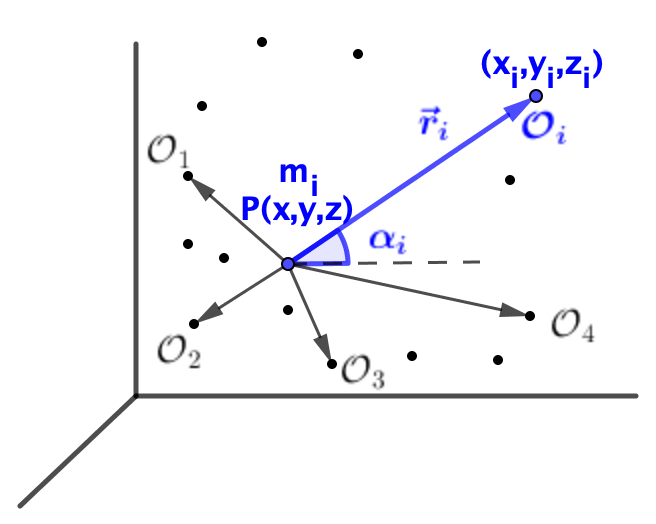
\includegraphics[width=.4\textwidth]{imagenes/imagenes05/T05IM07.png}
\end{figure}
\end{multicols}

$\vec F_{res}=\vec 0=-\vec {\grad} \mathcal E_p= $

$=\displaystyle \pdv{\mathcal E_p}{x} \ \vec i + \pdv{\mathcal E_p}{y} \ \vec j + \pdv{\mathcal E_p}{z} \ \vec k $

Fuerza que ejerce sobre la partícula $m$ el centro atractivo $\mathcal O_i$

$\vec F_i=\dfrac K r_i \vec u_i = \dfrac k {\sqrt{(x-x_i)^2+(y-t_i)^2+(z-z_i)^2}} \ \vec u_i=$

$\vec u_i= \vec i \ \cos \alpha_i + \vec j \ \cos \beta_i + \vec k \ \cos \gamma_i$

Componentes de $\vec u_i$, cosenos directores de $\vec r_i$:

$\cos \alpha_i=\dfrac {x-x_i}{\sqrt{(x-x_i)^2+(y-t_i)^2+(z-z_i)^2}}; $ análogamente $\cos \beta_i$ y $\cos \gamma_i$.

\begin{comment}
Ecuación extralarga, la corto como más abajo, con 'eqnarray*'
$\vec F_i=k  
\vec i \ \dfrac {x-x_i}{\sqrt{(x-x_i)^2+(y-t_i)^2+(z-z_i)^2}} + 
\vec j \ \dfrac {y-y_i}{\sqrt{(x-x_i)^2+(y-t_i)^2+(z-z_i)^2}} + 
\vec k \ \dfrac {z-z_i}{\sqrt{(x-x_i)^2+(y-t_i)^2+(z-z_i)^2}}  
$	
\end{comment}


\begin{eqnarray*}
\vec F & = & \vec i \ \dfrac {x-x_i}{\sqrt{(x-x_i)^2+(y-t_i)^2+(z-z_i)^2}} \ +  \nonumber \\
    & & \vec j \ \dfrac {y-y_i}{\sqrt{(x-x_i)^2+(y-t_i)^2+(z-z_i)^2}} \ + \nonumber \\
  & & \vec k \ \dfrac {z-z_i}{\sqrt{(x-x_i)^2+(y-t_i)^2+(z-z_i)^2}}  \ = \ \nonumber \\
  -\vec{\grad} \mathcal E_p &= & -\vec i \ \pdv{\mathcal E_p}{x}+ \vec j \ \pdv{\mathcal E_p}{y}+ \vec k \ \pdv{\mathcal E_p}{z}
\end{eqnarray*}


Como $\displaystyle \pdv{\mathcal E_p}{x}=0 \to \sum_{i=1}^N 
\dfrac {x-x_i}{\sqrt{(x-x_i)^2+(y-t_i)^2+(z-z_i)^2}}=0$

$\displaystyle  \to \sum_{i=1}^N x-x_i=0=\sum_{i=1}^N x - \sum_{i=1}^N x_i \to \ \ Nx-\sum_{i=1}^N x_i=0$

$\displaystyle Nx=\sum_{i=1}^N x_i \to \quad x=\dfrac 1 N \sum_{i=1}^N x_i$ y análgogamente para las otras coordenadas del punto de equilibrio.


Luego la posición de equilibrio de la partícula sometida a la acción de estos $N$ centros de atracción es:

$$ x= \dfrac 1 N \ \sum_{i=1}^N x_i; \quad y= \dfrac 1 N \ \sum_{i=1}^N y_i; \quad z= \dfrac 1 N \ \sum_{i=1}^N z_i$$




\newpage %**************************************

\begin{myblock}{Estática en la ingeniería.}

Las aplicaciones prácticas de la estática en la ingeniería son muy numerosas, siendo quizás la parte de la mecánica más empleada. Esto es así especialmente en la ingeniería civil y en el análisis estructural: por lo general las estructuras se diseñan para estar y permanecer en reposo bajo las cargas de servicio estáticas, o para que su movimiento bajo cargas dinámicas sea pequeño y estable (vibraciones).
	
\end{myblock}



